\let\negmedspace\undefined
\let\negthickspace\undefined
\documentclass[journal]{IEEEtran}
\usepackage[a5paper, margin=10mm, onecolumn]{geometry}
%\usepackage{lmodern} % Ensure lmodern is loaded for pdflatex
\usepackage{tfrupee} % Include tfrupee package

\setlength{\headheight}{1cm} % Set the height of the header box
\setlength{\headsep}{0mm}     % Set the distance between the header box and the top of the text

\usepackage{gvv-book}
\usepackage{gvv}
\usepackage{cite}
\usepackage{amsmath,amssymb,amsfonts,amsthm}
\usepackage{algorithmic}
\usepackage{graphicx}
\usepackage{textcomp}
\usepackage{xcolor}
\usepackage{txfonts}
\usepackage{listings}
\usepackage{enumitem}
\usepackage{mathtools}
\usepackage{gensymb}
\usepackage{comment}
\usepackage[breaklinks=true]{hyperref}
\usepackage{tkz-euclide} 
\usepackage{listings}
% \usepackage{gvv}                                        
\def\inputGnumericTable{}                                 
\usepackage[latin1]{inputenc}                                
\usepackage{color}                                            
\usepackage{array}                                            
\usepackage{longtable}                                       
\usepackage{calc}  
\usepackage{amsmath,amssymb}

\usepackage{multicol}                                         
\usepackage{hhline}                                           
\usepackage{ifthen}                                           
\usepackage{lscape}
\begin{document}

\bibliographystyle{IEEEtran}

\title{
%	\logo{
NCERT - 12.9.4.11

\large{EE1003}
%	}
}
\author{Homa Harshitha Vuddanti

(EE24BTECH11062)
}	

\maketitle

\bigskip

\renewcommand{\thefigure}{\theenumi}
\renewcommand{\thetable}{\theenumi}
\textbf{Question}: Find the particular solution of the differential equation $\brak{x^3+x^2+x+1}\frac{dy}{dx}=2x^2+x; y=1$ when $x=0$\\
\textbf{Theoretical Solution: }\\
Given,
\begin{align}
\frac{dy}{dx}=\frac{2x^2+x}{x^3+x^2+x+1}\\
\frac{dy}{dx}=\frac{2x^2+x}{\brak{x+1}\brak{x^2+1}}\\
\end{align}
Splitting into partial fractions,\\
\begin{align}
\frac{dy}{dx}&=\frac{2x^2+x}{\brak{x+1}\brak{x^2+1}}=\frac{1}{2\brak{x+1}}+\frac{3x-1}{2\brak{x^2+1}}\\
\int dy&=\int \frac{1}{2\brak{x+1}}dx+\int \frac{3x-1}{2\brak{x^2+1}}dx\\
y&=\frac{1}{2} \ln{\abs{x+1}}+\frac{3}{4}\ln{\abs{x^2+1}}-\frac{1}{2}\tan^{-1}x+c
\end{align}
Substituting \brak{0,1} in the equation, we get the value of $c=1$
\begin{align}
y&=\frac{1}{2} \ln{\abs{x+1}}+\frac{3}{4}\ln{\abs{x^2+1}}-\frac{1}{2}\tan^{-1}x+1
\end{align}


\textbf{Solving by Bilinear transformation :}
Applying Laplace transformation
\begin{align}
\mathcal{L}\brak{y^\prime}=\mathcal{L}\brak{\frac{2x^2+x}{x^3+x^2+x+1}}\\
\end{align}
Let 
\begin{align}
\mathcal{L}\brak{\frac{2x^2+x}{x^3+x^2+x+1}}&=X\brak{s}\\
sY\brak{s}-y\brak{0}&=X\brak{s}\\
sY\brak{s}&=X\brak{s}+1\label{eq:1}
\end{align}
From bilinear transformation,
\begin{align}
s=\frac{2}{h}\brak{\frac{1-z^{-1}}{1+z^{-1}}}
\end{align}
Substituting in \eqref{eq:1},
\begin{align}
Y\brak{s}-z^{-1}Y\brak{s}=\frac{h}{2}\brak{X\brak{s}+z^{-1}X\brak{s}+1+z^{-1}}
\end{align}
Applying inverse $\mathcal{Z}$-transformation,
\begin{align}
y_{n+1}-y_n&=\frac{h}{2}\brak{\frac{2x_{n+1}^2+x_{n+1}}{x_{n+1}^3+x_{n+1}^2+x_{n+1}+1}+\frac{2x_{n}^2+x_{n}}{x_{n}^3+x_{n}^2+x_{n}+1}+\delta[n+1]
+\delta[n]
}\\
x_{n+1}&=x_n+h
\end{align}
\textbf{Trapezoidal Rule:}\\
Area is given by
\begin{align}
\int_a^{b} f\brak{x}dx&\approx h\brak{\frac{1}{2}f\brak{a}+f\brak{x_1}+f\brak{x_2}+\dots +f\brak{x_{n-1}}+\frac{1}{2}f\brak{b}}\\
h&=\frac{b-a}{n}\\
A_{n+1}&=A_n+\frac{h}{2}\brak{f\brak{x_{n+1}+f\brak{x_n}}}
\end{align}
Substituting, we finally get
\begin{align}
y_{n+1}&=y_n+\frac{h}{2}\brak{\frac{2x_{n+1}^2+x_{n+1}}{x_{n+1}^3+x_{n+1}^2+x_{n+1}+1}+\frac{2x_{n}^2+x_{n}}{x_{n}^3+x_{n}^2+x_{n}+1}}\\
x_{n+1}&=x_n+h
\end{align}
\textbf{Plotting:}
Taking the initial point $\brak{x_0,y_0}$ as $\brak{0,1}$ and the value of $h=0.01$
\begin{figure}[h!]
   \centering
   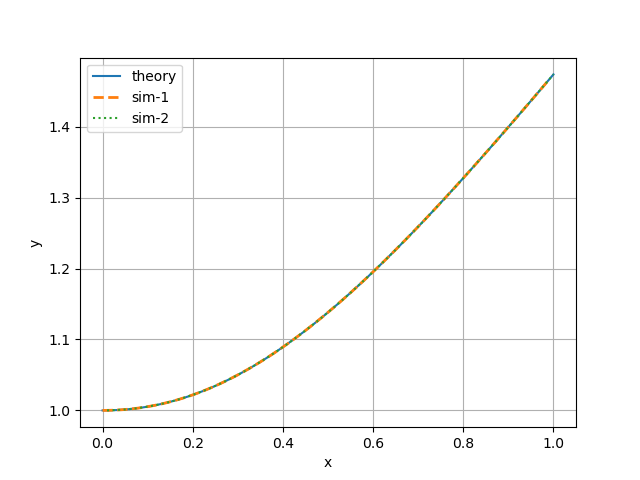
\includegraphics[width=1\columnwidth]{Figs/Figure_1.png}
   \caption{Plot}
\end{figure}
\end{document}


